\documentclass[a4paper,10pt,openright,oneside,notitlepage]{report}

\usepackage[utf8]{inputenc}
\usepackage[ngerman]{babel}
\usepackage{hyperref}
\usepackage[toc]{glossaries}
\usepackage[square, numbers]{natbib}
\usepackage{graphicx}
\usepackage{float}

\title{Anforderungsanalyse der Bachelorarbeit}
\author{Daniel Pollack}
\date{}

\newcommand{\ProgrammName}{ProgrammnamePlatzhalter}

\pdfinfo{
  /Title    (\title)
  /Author   (\author)
  /Creator  (\author)
  /Producer (\author)
  /Subject  ()
  /Keywords ()
}

\makeglossary


\begin{document}
\maketitle
\tableofcontents

\chapter{Einleitung}
\section{Anlass}
Die Idee zu diesem Bachelorthema ist aus dem Arbeitsalltag am Max-Plack Institut
für Biogeochemie in Jena entstanden. Durch Gespräche mit Kollegen und beim
\gls{Brainstorming} mit meinem Vorgesetzten bin ich zu dem Entschluss gekommen, 
dass das angestrebte Thema eine sinnvolle Ergänzung im Arbeitsalltag und eine
Verbesserung der Arbeitsabläufe, sowohl im Institut als auch anders wo
darstellt.

\section{Zweck}
Zweck dieser Arbeit soll es sein, eine Software zu entwickeln die den Aufbau und
die Wartung von Versuchsaufbauten beschleunigt und vor allem vereinfacht. Bei meiner Recherche stellte sich heraus, dass manche der am Institut
verwendeten Systeme lediglich von einer geringen Anzahl Personen konfiguriert und gewartet werden können. Dieser Zustand ist keineswegs optimal und kann, z.B. durch das Fernbleiben eben dieser Personen, den betrieblichen Ablauf erheblich stören.
\section{Ziele}
Diese Arbeit hat zum Ziel eine Softwarelösung zu entwickeln und umzusetzen, die 
es einem elektrotechnisch geschulten und in dem Umgang mit Computern geübten 
Nutzer erlaubt einen elektronischen Schaltkreis zu überwachen, zu messen und zu 
steuern. Dem Nutzer soll eine Möglichkeit geboten werden, mittels eines eingängigen Interfaces, Messungen an elektrotechnischen Schaltungen vor zu nehmen. Darüber hinaus soll die Erstellung von Schaltvorgängen in einer elektrotechnischen Schaltung ermöglicht werden.
\section{Referenzen}
Bei Recherchen verfestigte sich mein Eindruck, dass eine solche Software durch aus Potential hat, Wissenschaftlern und \gls{Maker}{Makern} das Leben und ihre Arbeit zu vereinfachen. So ist das Interesse an erschwinglicher Hardware und handlicher 
Software zum Prototyping und dem Aufbau von Versuchen besonders durch das 
Aufkommen des Arduinos gewachsen. D.~K.~Fisher und P.~J.~Gould~\cite{ModernInstrumentation} beschrieben in ihrem Paper einen 
Versuchsaufbau mit Hilfe eines Arduino-Nachbaus zur Ermittlung von 
Feuchtigkeitswerten in und um Pflanzen herum. Ihr Aufbau und vorallem die 
Software verfolgen ein ähnliches Prinzip wie das von mir angestrebte. Der 
Arduino dient ihnen alls Datenerfassungsergrät und übermittelt alle Daten ohne 
weitere Verarbeitung direkt an entweder ein Speichermedium oder an einen 
Server. In diesem und einigen anderen Papers geht es häufig auch um eine finanzielle Sicht auf Experimente und die damit verbundene Durchführbarkeit. So beschreibt \citet{joshua_m._pearce_open-source_2014} in Kapitel 4 seines Buches, wie er eine Feuchtigkeitskammer für seine Forschungsarbeit anschaffen wollte. Er beschreibt, das die kommerziell verfügbaren Produkte außerhalb des Finanzrahmens waren und man somit auch eine \acrshort{DYI}-Lösung zurückgreifen mussten. Herz dieser Lösung war, aufgrund seines Preises und der beständigen Unterstützung durch Software-Bibliotheken Dritter, der Arduino.

Der Aspekt einer Datenerfassung und Auswertung hat bereits andere veranlasst 
eine entsprechende Software zu erstellen. Einer der jüngeren Ansätze stammt 
aus der Universität Basel~\cite{Instrumentino} und umfasst eine Software 
(Instrumentino) mit deren Hilfe extra angefertigte Arduino-Sketche (Controlino) 
und eine problembezogen konfigurierte Oberfläche zum Einsatz kommen. 
Nach eindringlicher Analyse der Software und einem Versuch eine eigene 
Testkonfiguration mit der Software, mit Hilfe des Entwicklers, zu erstellen, bin 
ihc zu dem Schluss gekommen das diese Software nicht als ``fertig'' angesehen 
werden kann und nicht einsatzbereit ist. Der Entwickler weißt in einer 
\href{https://github.com/yoelk/Instrumentino/blob/master/documents/Instrumentino\%20presentation.pptx}{Präsentation} auch darauf hin das der Konfigurationsprozess einen "`Administrator/Entwickler"' benötigt und es nicht vorgesehen ist diesen Schritt einem Endnutzer zu überlassen. 
Ein ausgereiftes Konzept, wenn auch etwas älter stammt von \citet{dedrick_inexpensive_2000} und beschreibt einen Datenlogger auf Mikrocontrollerbasis mit einer entsprechenden Software zum Auslesen der gesammelten Daten. Auch hier wurde Wert auf den finanziellen Rahmen, sowie die Weiterverarbeitung und Langzeiterfassung von Daten gelegt.
\part{Programm}
\chapter{Übersicht}
\chapter{Funktionalitäten}
\chapter{Optionale Funktionalitäten}
\section{Usability}
\section{Verlässlichkeit Wartung}
\section{Leistung}
\section{Implementation \/ Umsetzung}
\section{Interface}
\section{Packaging}
\section{Lizenz / Rechtliches}
\chapter{Modelle}
\section{Szenarios}
\section{Use case model}
\section{Analysis object model}
\section{Dynamic model}
\section{User interface - navigation und Mockups}

\chapter{Modelle}
\section{Szenarios}
\subsection{Überwachung und Messung an einem Versuchsaufbau}
Angenommen jemand hat einen Versuchsaufbau mit mehreren Temperatur Sensoren des gleichen Types aufgebaut und will damit seine Wohnung, über die Dauer einer Woche, überwachen. Der Aufbau ist relativ schnell bewältigt und das größte Problem ist die Flut an Daten die bewältigt werden muss, wenn jede Minute ein Wert pro Sensor gespeichert werden soll. Darüber hinaus sollen die Daten so gespeichert werden, das eine spätere Auswertung, evtl. auch durch Dritte, nach gängigen Normen vorgenommen werden kann. Der Nutzer hat in seinem beruflichen Umfeld bereits Erfahrungen mit Elektrotechnik gesammelt und ist geübt im Umgang mit Computern und der Bedienung von Anwendungen.

Der Aufbau ist abgeschlossen und er sucht nur noch nach einer Software die seinen Bedürfnissen entspricht. Hier kommt die zu entwickelnde Software ins Spiel. Er startet die Software und konfiguriert  seine Messung mit Hilfe des Wizards nach seinen Vorstellungen. Er will das die Werte nicht nur generisch "A1", "`A2"' und so weiter heißen, sondern entsprechender des Raumes in dem sich der Sensor befindet beschriftet werden. Sofort sieht er in dem Wizard diese Option und trägt die Beschriftung der Pins in die vorgesehenen Textboxen ein. Da die Sensoren nur ein analoges Signal im Rahmen von 0 bis 5 Volt ausgeben und dieses Signal noch in Grad Celsius umgewandelt werden muss trägt er zu jedem Pin noch die entsprechende Übertragungsfunktion ein. Nachdem dies geschehen ist geht er in dem Wizard eine Schritt weiter und bekommt die Möglichkeit die digitalen Pins des Arduinos zu Steuern. Er entscheidet sich gegen die Nutzung. Es sollen lediglich Daten gemessen und geloggt werden. Auf der letzten Seite des Wizards bekommt er die Optionen zu Einrichtung des \acrshort{CSV}-Loggers. Da er die Software auf einer deutschsprachigen Maschine betreibt und die anschließende Auswertung auch in einer deutschsprachigen Tabelenbearbeitungssoftware geschehen wird, gibt er an, dass entsprechende Tausendertrenner und ähnliches verwendet werden sollen. Der Wizard hat ihm allerdings auf Grund der verwendeten System-Einstellungen diesen Vorschlag bereits unterbreitet. Der Nutzer gibt nur noch an das er sowohl die umgerechneten Temperaturen und die Spannungswerte in dem Log hinterlegt haben möchte. 

Nach dem die Konfiguration abgeschlossen ist, muss noch der Arduino-Sketch mittels der Arduino eigenen IDE installiert werden. Ist dies erfolgt kann die Messung beginnen. Der Nutzer bekommt nun in Echtzeit die gemessenen Werte angezeigt. Er kann selektiv nur einen oder mehrere Werte anzeigen lassen und zwischen den Spannungswerten und den umgerechneten Werten auswählen. Zusätzlich kann er sich noch eine Tendenz einblenden lassen, um etwa zu sehen wann und wo er vergessen hat ein Fenster zu schließen und somit der Raum auskühlt. 

Nun da die Messung läuft kann er sich anderen Dingen zu wenden und ggf. ab und zu nachschauen ob es interessante Veränderungen in den gemessen Werten gibt.
Nach Ablauf der einen Woche beendet er die Messung und kann nun die Werte mit Hilfe einer anderen Software genauer überprüfen.
\subsection{Steuerung und Messung an einem Versuchsaufbau}
Angenommen ein Nutzer verfügt über einen Versuchsaufbau um einen Luftentfeuchter zu betreiben. Dieser Aufbau benötigt die Option den Entfeuchtungsprozess ein und auszuschalten je nach Feuchtigkeit der ihn umgebenden Luft. Er hat eine genaue Vorstellung der Grenzwerte zum ein und ausschalten der Entfeuchters und beginnt folglich mit der Konfiguration einer entsprechenden Messung in der Software. Den benötigten Arduino hat er bereits an den Entfeutcher angeschlossen und alle notwendigen Pins mit ihren Konterparts verbunden. Die Software des Arduinos hat er mit Hilfe der IDE installiert. Gleitet wurde er dabei von einer, der Software beiliegenden Anleitung. Nun kann er die Software starten und mit der Konfiguration beginnen.
Mit Hilfe des Wizards benennt er die Signale die über die analogen Schnittstellen seines Arduinos gemessen werden und versieht sie zu gleich mit der von Sensorhersteller angegebenen Übertragungsfunktion. Hat er diesen Schritt beendet, kann er auf der nächsten Seite des Wizards bedingungen definieren um die Pumpe des Entfeuchters ein bzw. auszuschalten. Er verknüpft dafür die entsprechenden analogen Signale, wahlweise die Spannungswerte oder die übersetzten Werte mit einem entsprechenden digitalen Pin und bestimmt das Verhalten bei bestimmten Werten. Der Nutzer entscheidet sich den Entfeuchter abzuschalten wenn der relative Feutchtigkeitswert unter 50\% fällt. Diesen Wert hat er aus einem Wohnmagazin entnommen, mit dem Versprechend, dass diese Feuchtigkeit bei Wohn und Arbeitsräumen als angenehm empfunden wird bei einer Raumtemperatur von etwa 20 Grad Celsius. 

Nachdem die Bedingungen definieren sind, sieht der Nuzter die letzte Seite des Wizards und kann dort den Logger einstellen, da er eine gewissen Neugierde über den Feutigkeitsverlauf in dem Raum empfindet entscheidet er sich die Werte auch gleich mit zu loggen, in einem Rhythmus von 10 Minuten. 

Sobald diese letzte Option bearbeitet wurde startet der Nutzer die Messung. Nach einiger Zeit, 3 Tagen kommt er zurück und schaut sich die bis dahin gemessenen Werte an. Eine Auswertung kann er nun mit einem anderen Programm vollziehen und ggf. Konsequenzen in seinem Lüftungsverhalten o.ä. vornehmen.
\section{Use case model}
Dieses Use case Diagramm zeigt die dem Nutzer zu Verfügung stehen Optionen.
\begin{figure}[H]
 \centering
 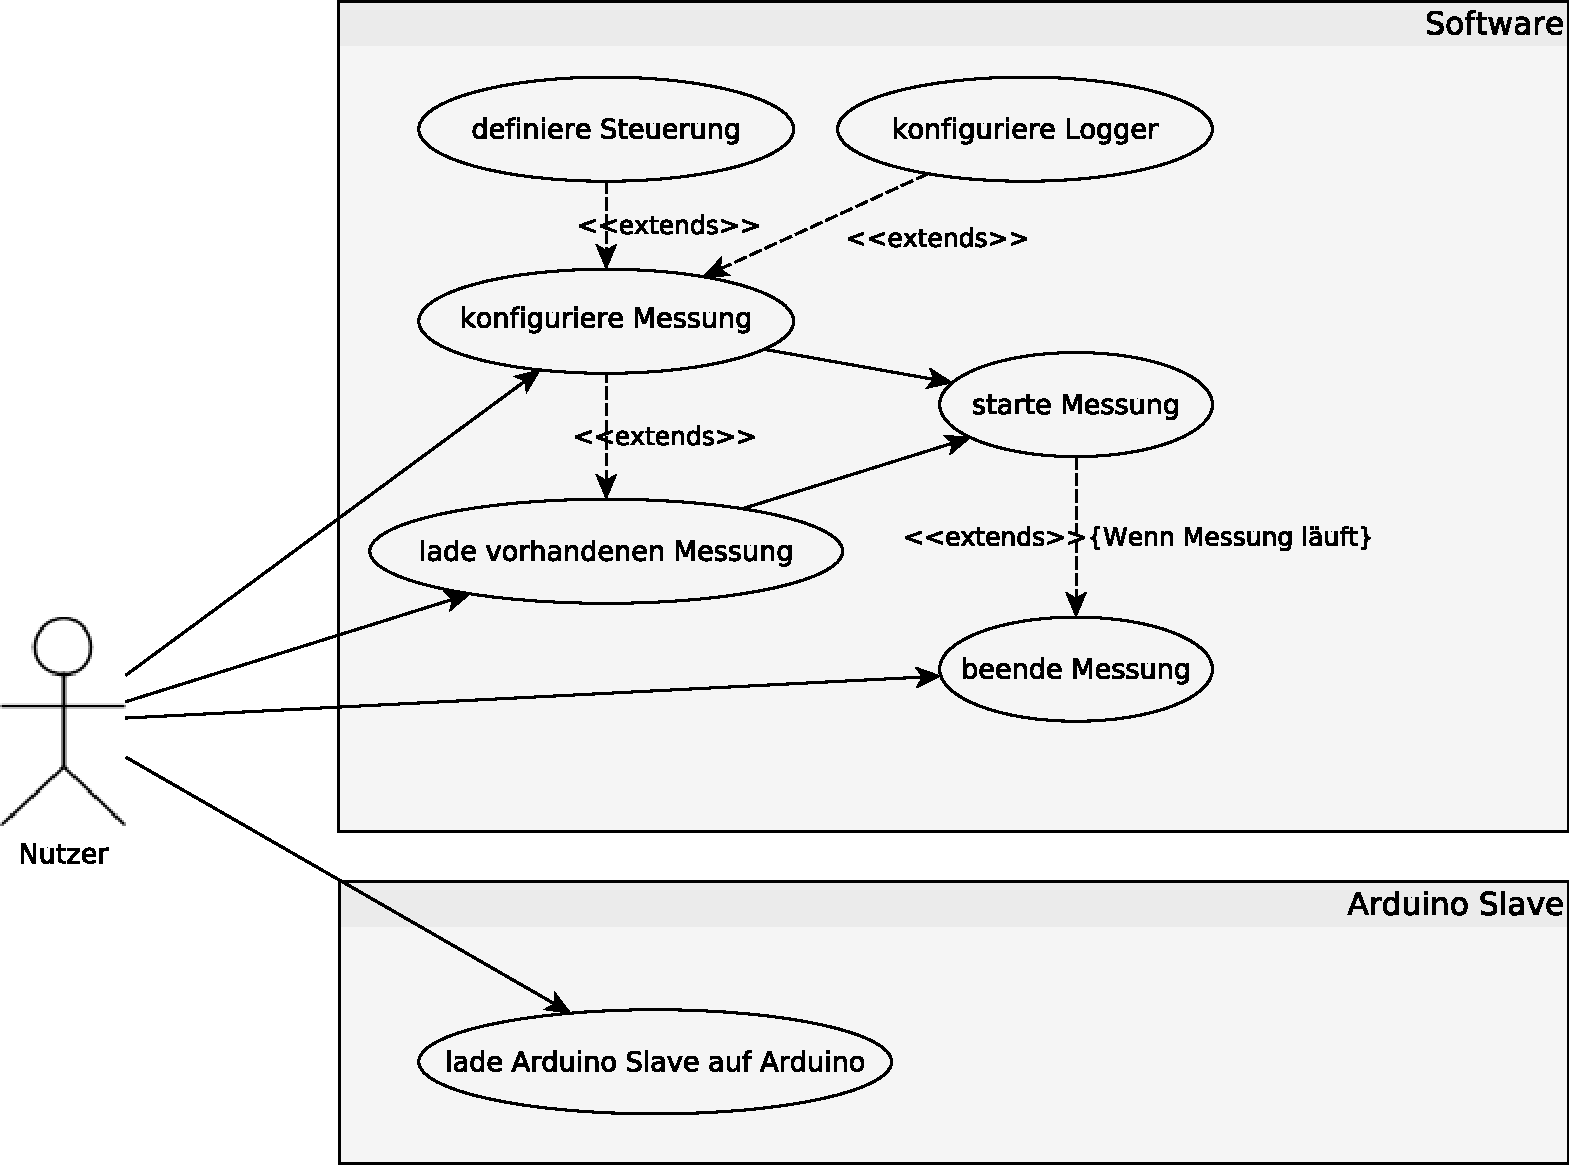
\includegraphics[width=\textwidth, keepaspectratio=true]{../Diagramme/BachelorUseCase1.pdf}
\end{figure}

%\section{Analysis object model}
%\section{Dynamic model}
\section{Flowchart}
Dieses Flowchart zeigt die notwendigsten Schritte, die von der Software und dem Nutzer unternommen werden müssen um eine erfolgreiche Messung durch führen zu können. 
\begin{figure}[H]
 \centering
 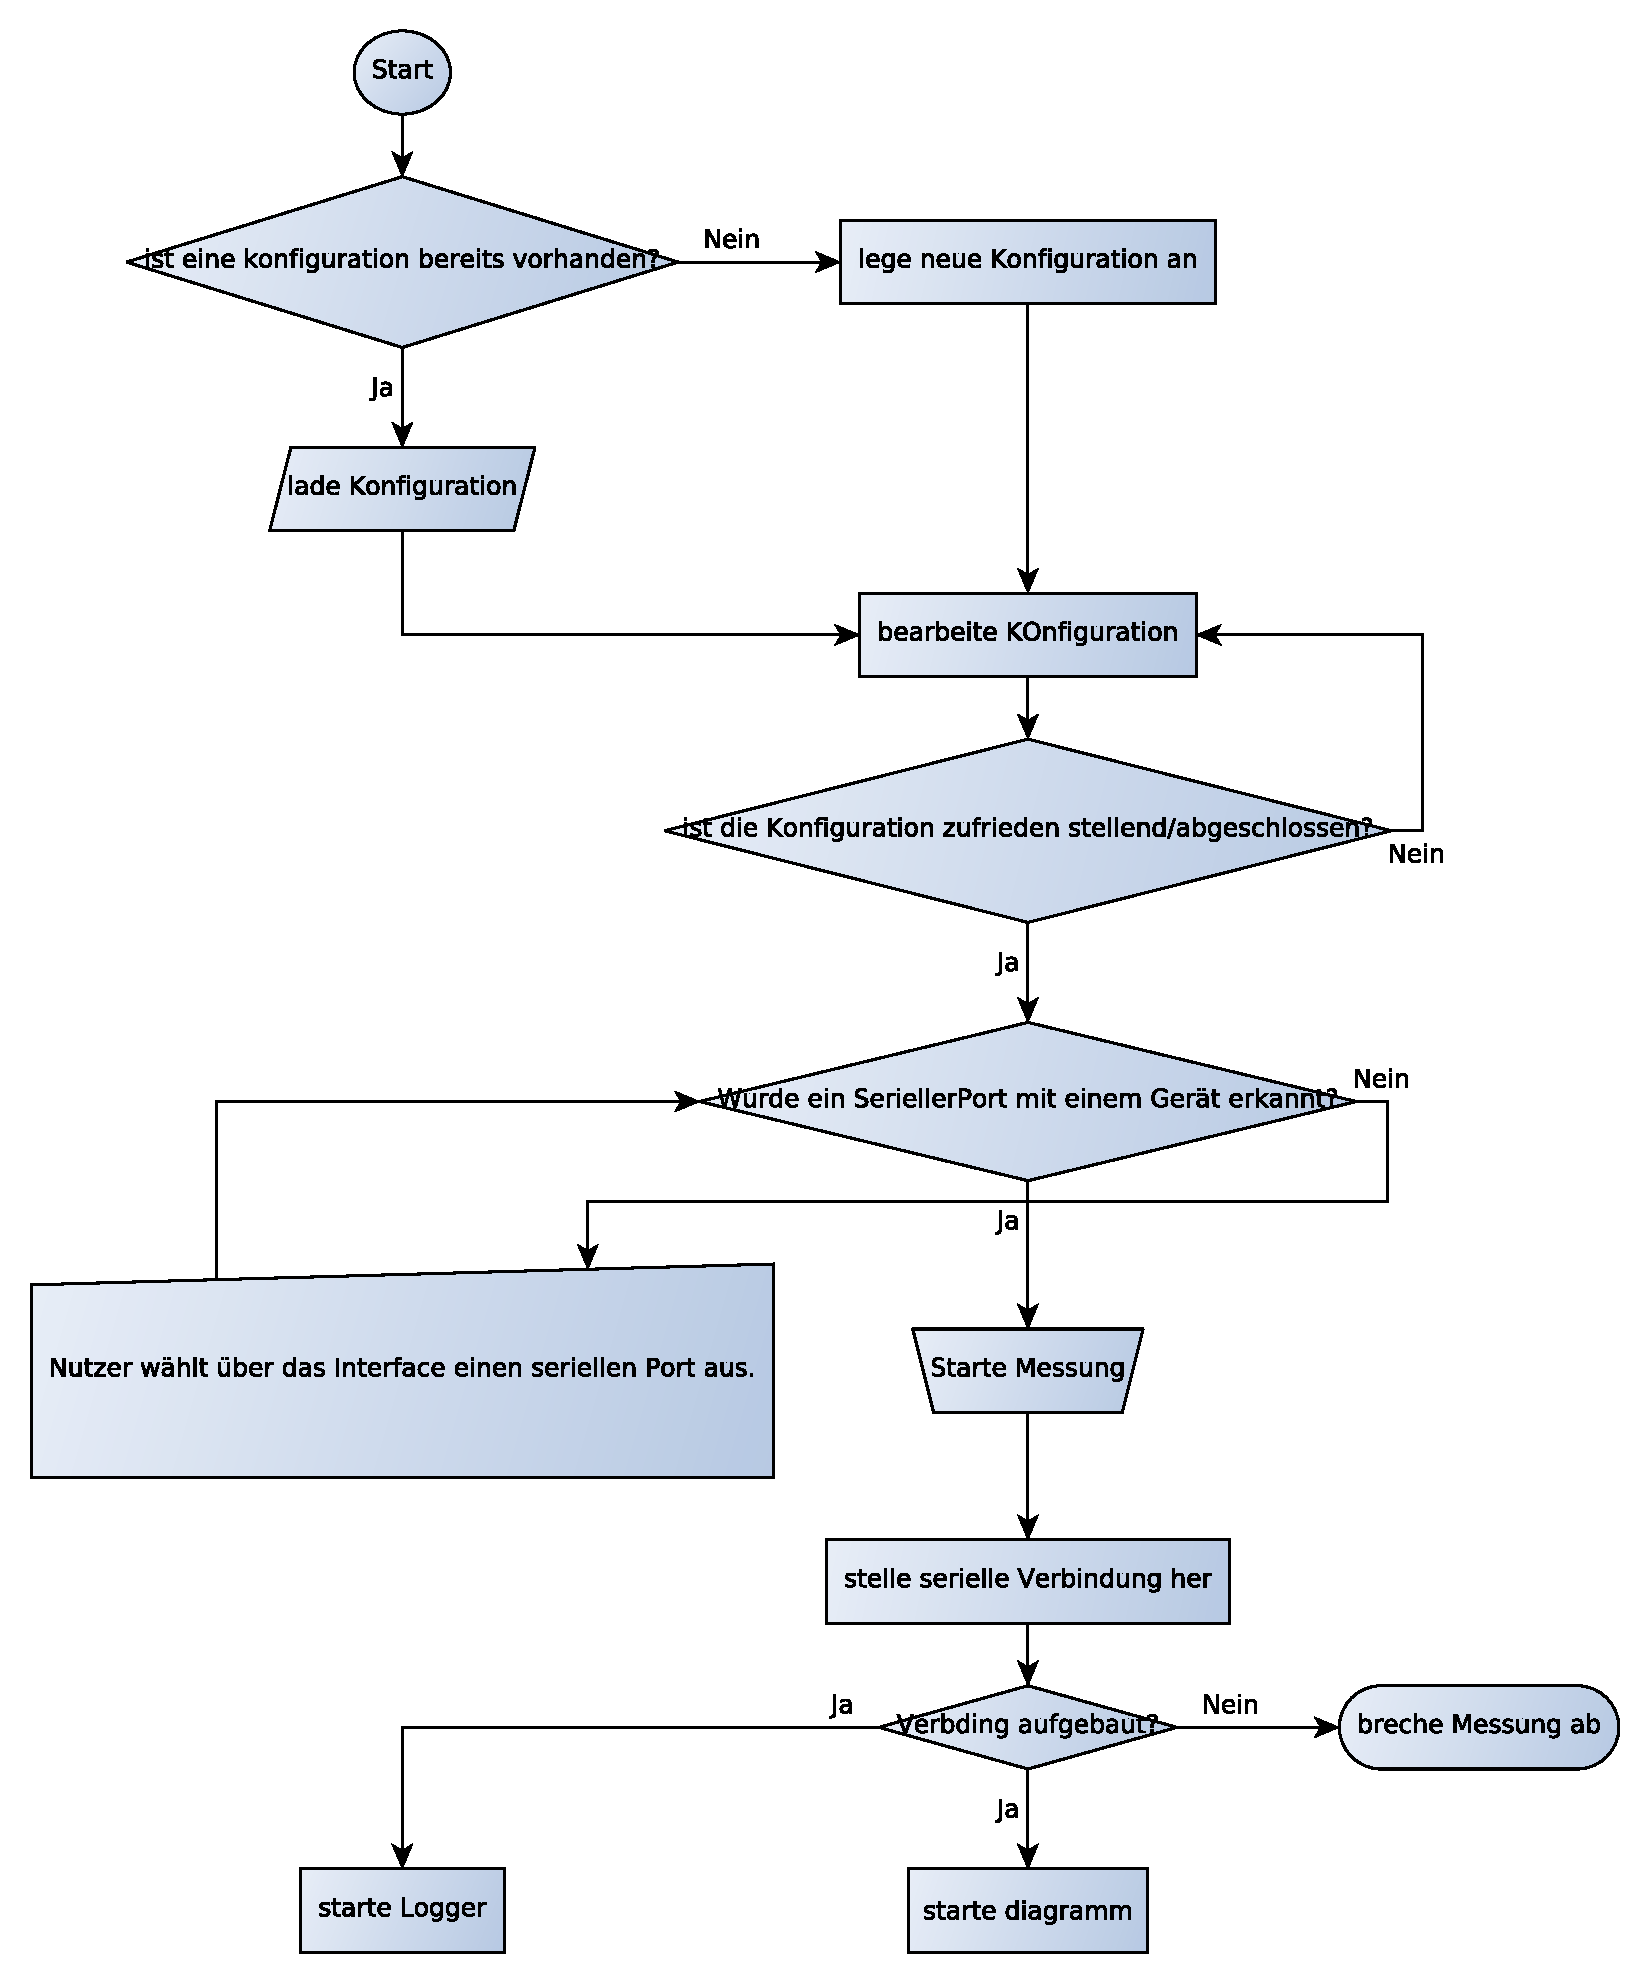
\includegraphics[width=\textwidth, keepaspectratio=true]{../Diagramme/SoftwareFlowChart.pdf}
\end{figure}
\section{Aufbau}
Ein UML-Diagramm zum Aufbau der Software befindet sich noch in der Entwicklung und wird in einer späteren Version dieses Dokumentes nachgereicht.
%grobes UML
\section{User Interface - Wireframe}
Ein Wireframe befindet sich gerade noch in der Erarbeitungsphase und wird in einer späteren Version dieses Dokuments nachgereicht.
%\addcontentsline{toc}{chapter}{Glossar}
\newglossaryentry{Brainstorming}{
name=Brainstorming,
description={Eine Methode zur Findung von neunen, ungewöhnlichen Ideen}
}
\newglossaryentry{Maker}{
name=Maker,
description={Eine Person die zu der 'Do-It-Yourselfe' Subkultur zählt und Geräte/Maschienen unter Einsatz moderner Technik herstellt}
}
\newglossaryentry{Eventlogging}{
name=Eventlogging,
description={Ermöglicht die Protokollierung von (vordefinierten) systembezogenen Event. Dies ist dienlich für die Analyse eines System}
}
\newglossaryentry{Uebertragungsfunktion}{
name=Übertragungsfunktion,
description={Eine Übertragungsfunktion beschreibt im naturwissenschftlichen Rahmen eine Funktionen die den Zusammenhang zwischen Eingangs und Ausgangssignal beschreibt}
}
\newacronym{FAQ}{FAQ}{Frequently Asked Questions}

\newglossaryentry{CSV-detail}{
name={Comma-separated values},
description={Ein plain-text Format, in dem Werte durch Kommata getrennt gespeichert werden}
}
\newacronym[see={[Glossary:]{CSV-detail}}]{CSV}{CSV}{Comma-separated values\glsadd{CSV-detail}}
\printglossaries

\addcontentsline{toc}{chapter}{Bibliography}
\bibliographystyle{plainnat}
\bibliography{Bibliography}


\end{document}
